\documentclass{article}
\usepackage{amsmath, amssymb, amsfonts}
\usepackage{fullpage}
\usepackage{enumerate}
\usepackage{graphicx}

\title{CS 4780/5780 Homework 9\vspace{-10pt}}
\author{Due: Tuesday 05/08/18 11:55pm on Gradescope}
\date{}

\begin{document}
    \maketitle
    \section*{Problem 1: Gaussian Process Regression} 
    Consider you have the following dataset: 
    \begin{table}[h]
    \centering
    \begin{tabular}{|c|c|c|}
        \hline
        No.& $\mathcal{X}$ & $\mathcal{Y}$ \\
        \hline
        1 & -1 & 5 \\
        2 & 1 & 5 \\
        3 & 2 & 8 \\
        \hline
    \end{tabular}
    \end{table}
    \newline
    and you are going to use a Gaussian Process
    $$f(x) \sim GP (m, k)$$ to model the underlying relationship between $\mathcal{X}$ and $\mathcal{Y}$. 
    After discussing with the professors, you decide to use a zero mean function and a quadratic kernel 
    for your GP, namely, 

    $$m(x) = 0$$
    $$k(x, x') = (x \cdot x' + 1)^2$$

    \begin{enumerate}[(a)]
        \item What is the mean and covariance of your GP prior? Please use the order provided to compute
        the mean and the covariance of the prior, e.g., the (1,2)-th entry of the 
        covariance matrix should be $k(-1, 1)$. 
        \item Now, you are given the following test points:
            \begin{table}[h]
                \centering
                \begin{tabular}{|c|c|c|}
                    \hline
                    No.& $\mathcal{X}$ & $\mathcal{Y}$ \\
                    \hline
                    1 & -2 & 8 \\
                    2 & 0 & 4 \\
                    \hline
                \end{tabular}
               \end{table}
        \newline
        Assume a noise free setup. What is the mean and covariance of your GP posterior? 
        Does the mean of your GP posterior match with your the target values of your test point? 
    \end{enumerate}
    \newpage
    \section*{Problem 2: RELU-network}
    In this question, you are going to explore a 2-layer
    fully connected network with RELU activation function. 
    \begin{figure}[h!]
        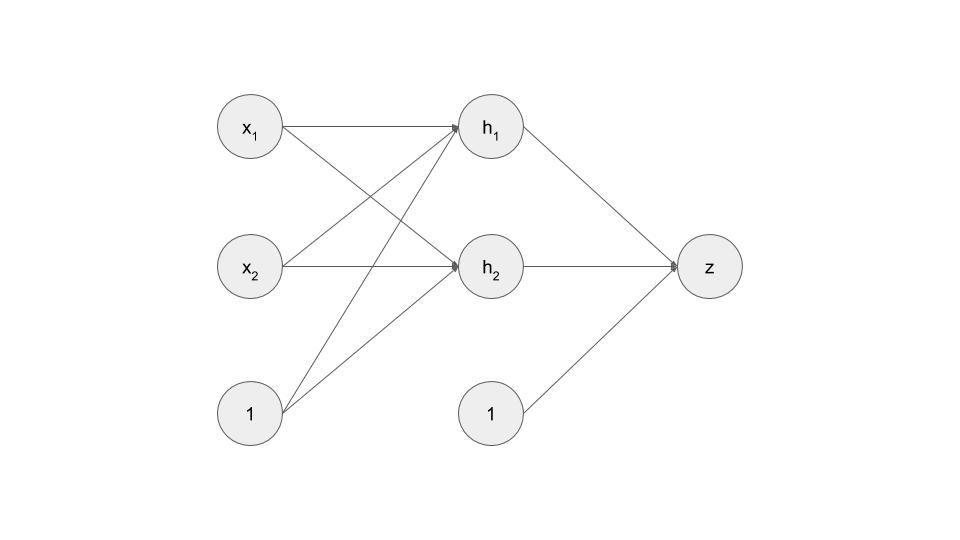
\includegraphics[width=\textwidth]{nn.jpg}
    \end{figure}
    \newline
    Suppose you have the architecture above, namely, 
    \begin{align*}
        \begin{bmatrix}h_1 \\ h_2 \end{bmatrix} &= \begin{bmatrix}w_{11} & w_{12} & w_{13} \\w_{21} & w_{22} & w_{23}\end{bmatrix} \begin{bmatrix} x_1 \\ x_2 \\ 1\end{bmatrix} \\
        z &= \begin{bmatrix} v_1 & v_2 & v_3\end{bmatrix} \begin{bmatrix}
        f(h_1) \\ f(h_2) \\ 1 
        \end{bmatrix}  \\
        t &= \sigma(z) 
    \end{align*}
    where $f(h_i) = max(0, h_i)$, $\sigma(z) = \frac{1}{1 + e^{-z}}$ and $t$ is the output of the network.

    \begin{enumerate}[(a)]
        \item Suppose $\begin{bmatrix}w_{11} & w_{12} & w_{13} \\w_{21} & w_{22} & w_{23}\end{bmatrix} = \begin{bmatrix}1 & -1 & 0 \\-1 & -1 & 0\end{bmatrix}$ and $\begin{bmatrix} v_1 & v_2 & v_3\end{bmatrix} = \begin{bmatrix} 1 & 1 & -2\end{bmatrix}$. Draw the decision boundary of the network, namely, $\sigma(z) = 0.5$ within the range $[-10, 10] \times [-10, 10]$. Please indicate the positive and negative side of the boundary. 
        \item Assume the weights in (a), what is the prediction for $[x_1, x_2]^T = [1,1]^T$?
        \item Usually, the weights $W = \begin{bmatrix}w_{11} & w_{12} & w_{13} \\w_{11} & w_{12} & w_{13}\end{bmatrix}$ and $V = \begin{bmatrix} v_1 & v_2 & v_3\end{bmatrix}$have to be learned using Stochastic Gradient Descent. For neural network binary classification, a common loss function is the cross entropy loss
        $$l(y, t) = - (y \log (t) + (1 -y) \log (1-t))$$ where $y$ is the true label for a sample and $t$ is the output of the neural network. In order to use SGD, we have to derive the gradient with respect to $W$ and $V$. Show that for a single training example, $x = [x_1, x_2]$
        \begin{align*}
            \frac{\partial l}{\partial v_i} &= (t - y) f(h_i) \text{ for } i \neq 3 \\
            \frac{\partial l}{\partial v_3} &= (t - y) \\
            \frac{\partial l}{\partial w_{ij}} &= (t - y) v_i \mathbb{I}(h_i > 0) x_j \text{ for } j \neq 3\\
            \frac{\partial l}{\partial w_{i3}} &= (t - y) v_i \mathbb{I}(h_i > 0) 
        \end{align*}
        where $\mathbb{I}(\cdot)$ is the indicator function. 
    \end{enumerate}
\end{document}